\section{Consideraciones iniciales}

El presente trabajo utiliza la norma APA 6ª edición para la citación de referencias bibliográficas. Todas las citaciones a lo largo del texto utilizan hipervínculos hacia sus entradas correspondientes en \hyperref[chap:referencias]{Referencias bibliográficas} de la página~\pageref{chap:referencias}. Muchos términos científicos utilizados se ha optado por escribirlos en inglés, ya que son ampliamente conocidos y usados en su forma original inglesa en el ámbito científico hispanohablante (como \emph{machine learning} \emph{deep learning}), mientras otros se encuentran en español por haberse considerado la forma más común (como \emph{inteligencia artificial} o \emph{red neuronal artificial}). En todo caso, se ha ofrecido una traducción de todos los términos ingleses para facilitar la lectura. Los términos utilizados repetidamente a lo largo del texto se encuentran en forma de acrónimos, los cuales se han explicitado en su primer uso y en los lugares donde ha sido necesario para mantener la claridad del texto. El significado de estos acrónimos puede consultarse en el glosario de la página~\pageref{chap:glosario}, al cual apuntan todos ellos por medio de hipervínculos.

Eventualmente, se incluyen códigos QR que enlazan a vídeos, audios u otros recursos de interés (p. ej., en la Figura \ref{fig:chatgpt_zero_shot_vs_few_shot}). Estos códigos pueden ser escaneados con cualquier dispositivo móvil, aunque también incluyen enlaces para su acceso desde el propio lector de PDF. Estos recursos son accesorios al texto y pueden cambiar o desaparecer con el tiempo. Por ello, en el Anexo \ref{anexo:repositorio} se incluye un enlace al repositorio de GitHub donde se aloja el código fuente de este trabajo, escrito en \defaultLaTeX{}, y la versión actualizada de este PDF.

Como resultados colaterales de este estudio, se ha creado un software para la generación de código musical en vivo, \emph{AI Muse}, que se expone en el capítulo \ref{chap:ai_muse}, y una obra de arte sonoro, \emph{AlgorAI}, sobre la cual tratamos en el capítulo \ref{chap:algorai} y en el anexo \ref{anexo:algorai}.

Por último, el título de este trabajo, hace un claro guiño a las ya cientos de publicaciones científicas que utilizan la expresión <<All You Need>> en el título (véase la Figura \ref{fig:all_you_need_publicaciones}). Esta expresión se ha convertido en un icono de los avances en \gls{ia}, especialmente desde la publicación del emblemático artículo \emph{Attention Is All You Need} \citep{vaswaniAttentionAllYou2017}. El lector curioso puede encontrar una lista actualizada de estas publicaciones en el repositorio de GitHub \emph{Awesome "all you need" papers} \citep{nishiKentoNishiAwesomeallyouneedpapers2024}.


\begin{figure}[H]
    \caption[Número de publicaciones científicas del campo de la inteligencia artificial por mes que contienen la expresión <<All You Need>> en su título]{Número de publicaciones científicas del campo de la inteligencia artificial por mes, hasta el 21 de enero de 2024, que contienen la expresión <<All You Need>> en su título.}
    \centering
    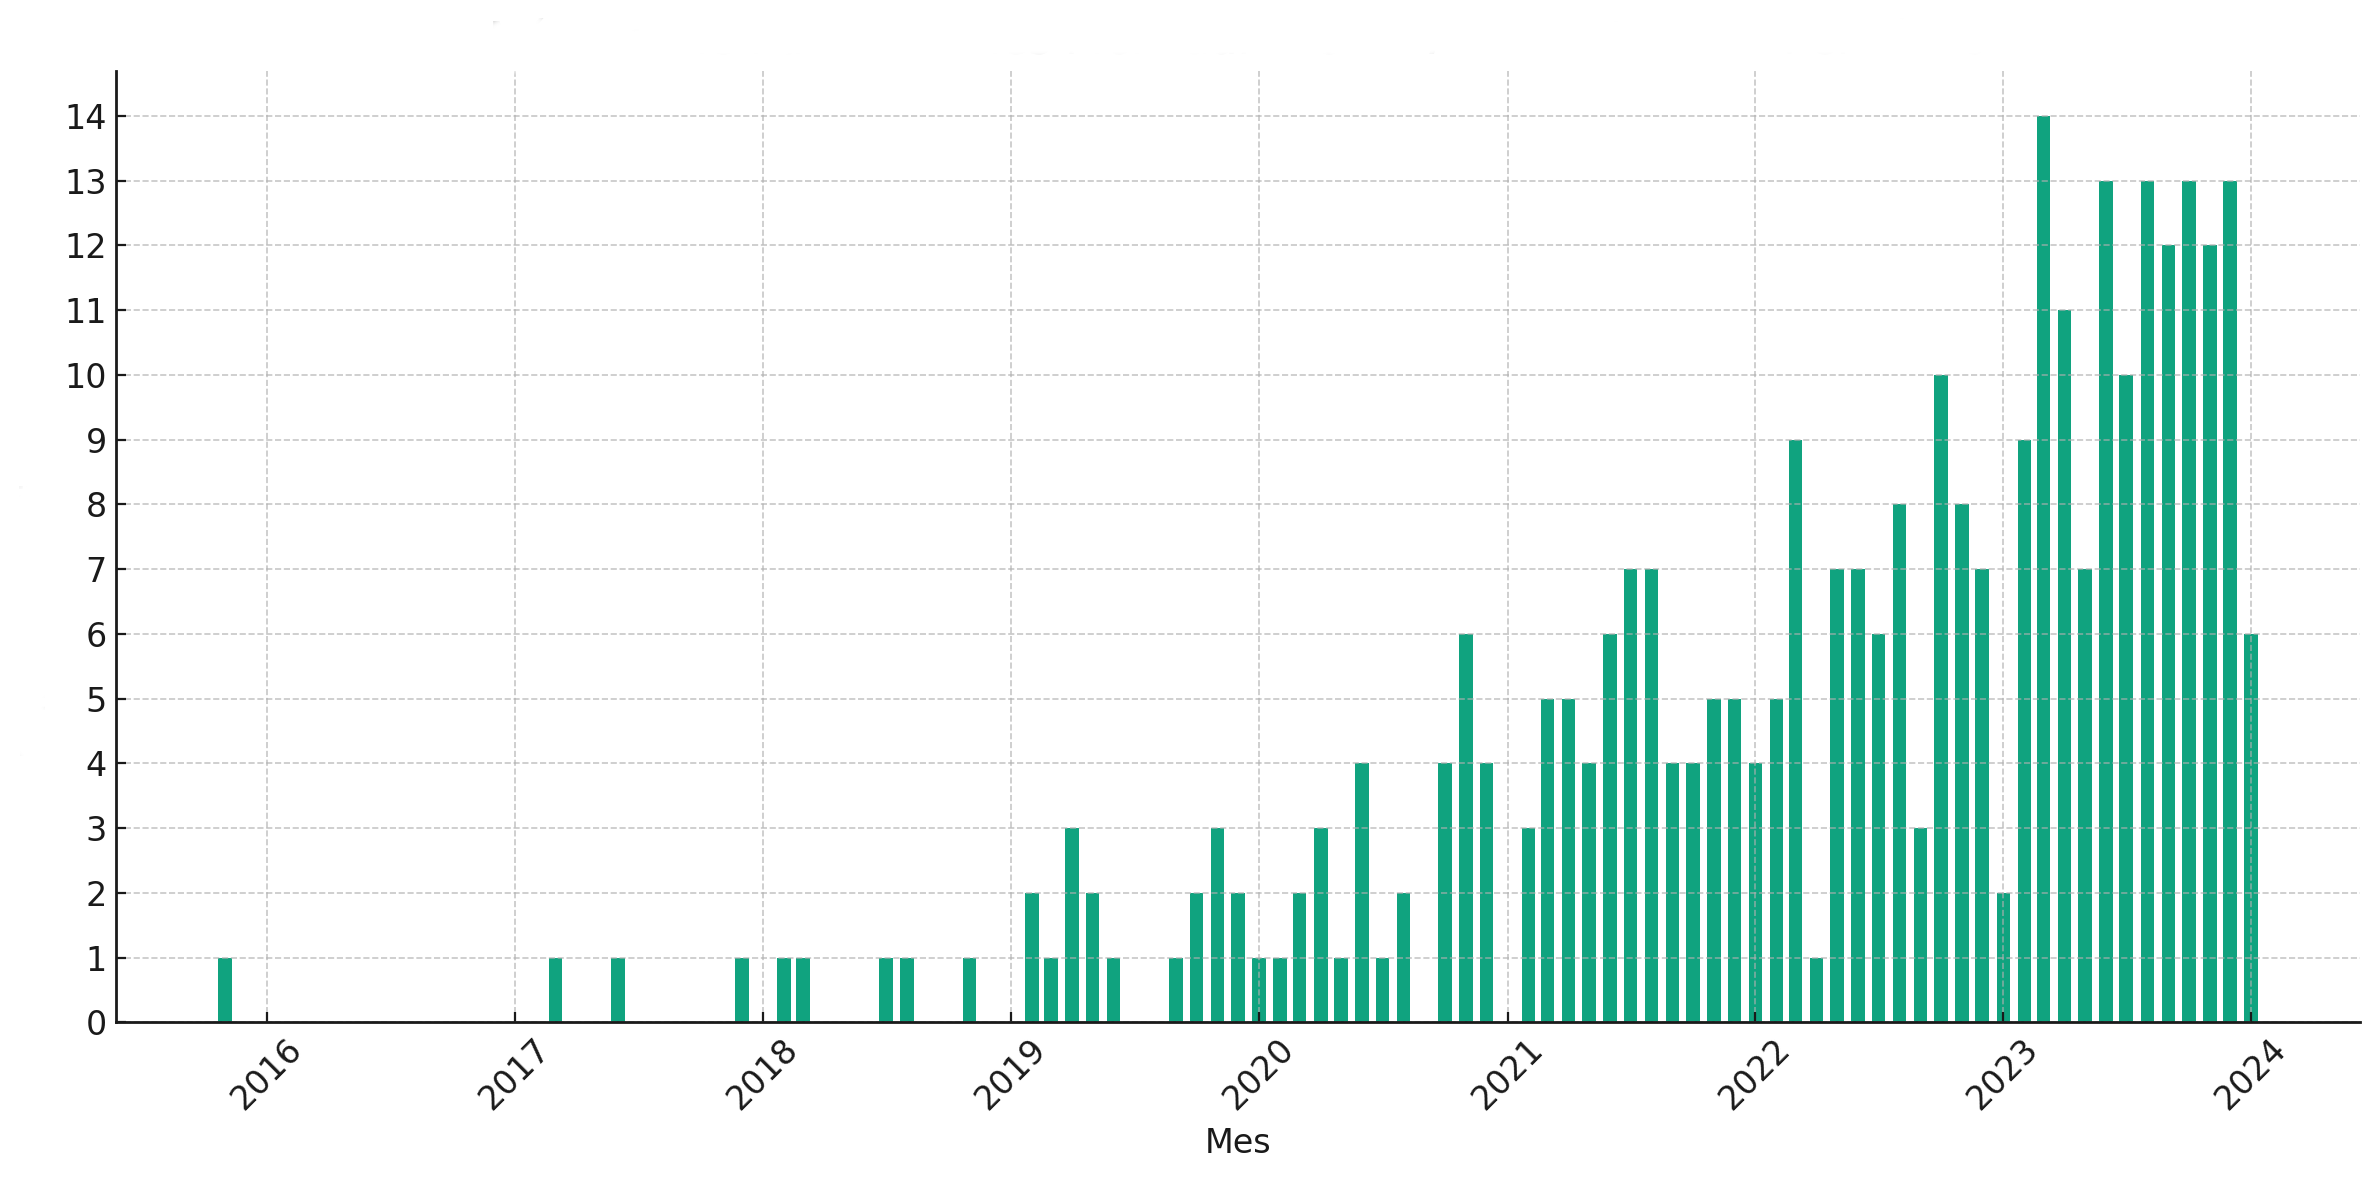
\includegraphics[width=0.7\textwidth]{./figuras/all_you_need_publicacionies_mensuales.png}
    \source{\propio\ a partir del listado de \cite{nishiKentoNishiAwesomeallyouneedpapers2024}}
    \label{fig:all_you_need_publicaciones}
\end{figure}



